\documentclass[11pt, a4paper]{report}

% ========== Common Packages ==========
\usepackage{fontspec}
\usepackage{kotex}
\usepackage{amsmath, amssymb, amsthm}
\usepackage{mathtools}
\usepackage{bm}
\usepackage{graphicx}
\usepackage{booktabs}
\usepackage{array}
\usepackage{tabularx}
\usepackage{longtable}
\usepackage{hyperref}
\usepackage{cleveref}
\usepackage{geometry}
\usepackage{fancyhdr}
\usepackage{titlesec}
\usepackage{enumitem}
\usepackage{xcolor}
\usepackage{tcolorbox}
\usepackage{algorithm}
\usepackage{algorithmic}
\usepackage{tikz}
\usetikzlibrary{arrows.meta, positioning, calc, decorations.pathreplacing, shapes.geometric, fit, patterns, angles, quotes, trees}
\usepackage{pgfplots}
\pgfplotsset{compat=1.18}
\usepackage{caption}
\usepackage{subcaption}
\usepackage{float}

\geometry{margin=2.5cm, top=3cm, bottom=3cm}

\usepackage{multirow}
\usepackage{siunitx}
% ========== Colors ==========
% Common
\definecolor{defblue}{RGB}{30, 80, 150}
\definecolor{thmgreen}{RGB}{20, 110, 60}
\definecolor{noteorange}{RGB}{200, 100, 0}
\definecolor{lightblue}{RGB}{230, 240, 255}
\definecolor{lightgreen}{RGB}{230, 255, 235}
\definecolor{lightorange}{RGB}{255, 245, 230}
\definecolor{lightgray}{RGB}{245, 245, 245}
% Extended
\definecolor{lightred}{RGB}{255, 235, 235}
\definecolor{darkred}{RGB}{180, 30, 30}
\definecolor{biogreen}{RGB}{10, 130, 80}
\definecolor{cvpurple}{RGB}{100, 40, 150}
\definecolor{injuryred}{RGB}{200, 40, 40}
\definecolor{codegray}{RGB}{240, 240, 245}
\definecolor{pipeblue}{RGB}{25, 100, 180}
\definecolor{constraintred}{RGB}{200, 50, 50}
\definecolor{termblack}{RGB}{30, 30, 30}
\definecolor{goldcolor}{RGB}{180, 140, 20}

% ========== Theorem-like environments ==========
\theoremstyle{definition}
\newtheorem{definition}{Definition}[chapter]
\newtheorem{example}{Example}[chapter]

\theoremstyle{plain}
\newtheorem{theorem}{Theorem}[chapter]
\newtheorem{proposition}{Proposition}[chapter]

\theoremstyle{remark}
\newtheorem{remark}{Remark}[chapter]

% ========== tcolorbox environments ==========
% --- Common (all parts) ---
\newtcolorbox{keyidea}[1][]{
  colback=lightblue,
  colframe=defblue,
  fonttitle=\bfseries,
  title={Key Idea},
  #1
}

\newtcolorbox{importantnote}[1][]{
  colback=lightorange,
  colframe=noteorange,
  fonttitle=\bfseries,
  title={Important},
  #1
}

\newtcolorbox{summary}[1][]{
  colback=lightgreen,
  colframe=thmgreen,
  fonttitle=\bfseries,
  title={Summary},
  #1
}

% --- Warning/Error ---
\newtcolorbox{warningbox}[1][]{
  colback=lightred,
  colframe=darkred,
  fonttitle=\bfseries,
  title={Warning},
  #1
}

% --- Domain: Biomechanics & Clinical ---
\newtcolorbox{clinicalnote}[1][]{
  colback=lightred,
  colframe=darkred,
  fonttitle=\bfseries,
  title={Clinical Note},
  #1
}

\newtcolorbox{biomechbox}[1][]{
  colback=lightgreen,
  colframe=biogreen,
  fonttitle=\bfseries,
  title={Biomechanics},
  #1
}

\newtcolorbox{injurybox}[1][]{
  colback={injuryred!8},
  colframe=injuryred,
  fonttitle=\bfseries,
  title={Injury Risk},
  #1
}

% --- Domain: Computer Vision ---
\newtcolorbox{cvbox}[1][]{
  colback={cvpurple!5},
  colframe=cvpurple,
  fonttitle=\bfseries,
  title={Computer Vision},
  #1
}

% --- Pipeline & Setup ---
\newtcolorbox{setupbox}[1][]{
  colback=lightgray,
  colframe=gray!60,
  fonttitle=\bfseries,
  title={Setup},
  #1
}

\newtcolorbox{pipelinebox}[1][]{
  colback=pipeblue!5,
  colframe=pipeblue,
  fonttitle=\bfseries,
  title={Pipeline Step},
  #1
}

\newtcolorbox{codebox}[1][]{
  colback=codegray,
  colframe=gray!70,
  fonttitle=\bfseries\ttfamily,
  title={Code},
  #1
}

\newtcolorbox{termbox}[1][]{
  colback=termblack!5,
  colframe=termblack!60,
  fonttitle=\bfseries\ttfamily,
  title={Terminal},
  #1
}

% --- Research ---
\newtcolorbox{hypothesis}[1][]{
  colback=goldcolor!8,
  colframe=goldcolor,
  fonttitle=\bfseries,
  title={Hypothesis},
  #1
}

\newtcolorbox{resultbox}[1][]{
  colback=thmgreen!8,
  colframe=thmgreen,
  fonttitle=\bfseries,
  title={Expected Result},
  #1
}

% --- Constraints & Solutions ---
\newtcolorbox{constraintbox}[1][]{
  colback=constraintred!8,
  colframe=constraintred,
  fonttitle=\bfseries,
  title={Constraint},
  #1
}

\newtcolorbox{solutionbox}[1][]{
  colback=thmgreen!8,
  colframe=thmgreen,
  fonttitle=\bfseries,
  title={Solution},
  #1
}

\newtcolorbox{databox}[1][]{
  colback=pipeblue!5,
  colframe=pipeblue,
  fonttitle=\bfseries,
  title={Data Spec},
  #1
}

% --- Progress/Status ---
\newtcolorbox{successbox}[1][]{
  colback=lightgreen,
  colframe=thmgreen,
  fonttitle=\bfseries,
  title={Success},
  #1
}

\newtcolorbox{nextbox}[1][]{
  colback=lightorange,
  colframe=noteorange,
  fonttitle=\bfseries,
  title={Next Step},
  #1
}

% --- Fitting guide ---
\newtcolorbox{failbox}[1][]{
  colback=lightred,
  colframe=darkred,
  fonttitle=\bfseries,
  title={Failure Pattern},
  #1
}

\newtcolorbox{fixbox}[1][]{
  colback=lightgreen,
  colframe=thmgreen,
  fonttitle=\bfseries,
  title={Fix},
  #1
}

\newtcolorbox{lessonbox}[1][]{
  colback=lightorange,
  colframe=noteorange,
  fonttitle=\bfseries,
  title={Lesson Learned},
  #1
}

% --- Specification ---
\newtcolorbox{specbox}[1][]{
  colback=cvpurple!5,
  colframe=cvpurple,
  fonttitle=\bfseries,
  title={Specification},
  #1
}

\newtcolorbox{checklistbox}[1][]{
  colback=lightgreen,
  colframe=biogreen,
  fonttitle=\bfseries,
  title={Checklist},
  #1
}

% ========== Custom math commands ==========
% Vectors (lowercase)
\newcommand{\vx}{\mathbf{x}}
\newcommand{\vd}{\mathbf{d}}
\newcommand{\vo}{\mathbf{o}}
\newcommand{\vc}{\mathbf{c}}
\newcommand{\vr}{\mathbf{r}}
\newcommand{\vp}{\mathbf{p}}
\newcommand{\vv}{\mathbf{v}}
\newcommand{\vn}{\mathbf{n}}
\newcommand{\vu}{\mathbf{u}}
\newcommand{\vt}{\mathbf{t}}
\newcommand{\ve}{\mathbf{e}}
\newcommand{\vq}{\mathbf{q}}
% Vectors (uppercase)
\newcommand{\vF}{\mathbf{F}}
\newcommand{\vM}{\mathbf{M}}
\newcommand{\va}{\mathbf{a}}
\newcommand{\vg}{\mathbf{g}}
\newcommand{\vX}{\mathbf{X}}
% Bold Greek
\newcommand{\vmu}{\bm{\mu}}
\newcommand{\vbeta}{\bm{\beta}}
\newcommand{\vtheta}{\bm{\theta}}
\newcommand{\vpsi}{\bm{\psi}}
% Matrices
\newcommand{\mSigma}{\bm{\Sigma}}
\newcommand{\mR}{\mathbf{R}}
\newcommand{\mS}{\mathbf{S}}
\newcommand{\mW}{\mathbf{W}}
\newcommand{\mJ}{\mathbf{J}}
\newcommand{\mG}{\mathbf{G}}
\newcommand{\mT}{\mathbf{T}}
\newcommand{\mI}{\mathbf{I}}
\newcommand{\mB}{\mathbf{B}}
\newcommand{\mK}{\mathbf{K}}
\newcommand{\mP}{\mathbf{P}}
\newcommand{\mF}{\mathbf{F}}
\newcommand{\mE}{\mathbf{E}}
\newcommand{\mA}{\mathbf{A}}
\newcommand{\mH}{\mathbf{H}}
% Sets and groups
\newcommand{\RR}{\mathbb{R}}
\newcommand{\SO}{\mathrm{SO}}
% Units
\newcommand{\degps}{\,\text{deg/s}}
\newcommand{\Nm}{\ensuremath{\,\text{N}\cdot\text{m}}}
\newcommand{\BW}{\,\text{BW}}

% ========== Header/Footer ==========
\pagestyle{fancy}
\fancyhf{}
\fancyhead[L]{\leftmark}
\fancyhead[R]{\thepage}
\renewcommand{\headrulewidth}{0.4pt}

% ========== Title formatting ==========
\titleformat{\chapter}[display]
  {\normalfont\huge\bfseries\color{defblue}}
  {\chaptertitlename\ \thechapter}{20pt}{\Huge}

\titleformat{\section}
  {\normalfont\Large\bfseries\color{defblue!80!black}}
  {\thesection}{1em}{}

\titleformat{\subsection}
  {\normalfont\large\bfseries\color{defblue!60!black}}
  {\thesubsection}{1em}{}


\begin{document}

\begin{titlepage}
\centering
\vspace*{1.5cm}
{\Large\color{gray} Final Experiment Log}
\vspace{0.5cm}

{\Huge\bfseries\color{defblue} 2026년 4월 13일\\[0.3cm]
Conda 환경 분리 $\rightarrow$ U-HMR 전체 프레임\\[0.3cm]
$\rightarrow$ GART 첫 실행}

\vspace{1cm}

{\LARGE\color{defblue!70!black} U-HMR 999프레임 4뷰 추론 완료\\
GART 3DGS 학습 첫 성공\\
OpenPose 마스킹 재추출 + Smoothing}

\vspace{2cm}
{\large 2026년 4월 13일}
\end{titlepage}

\tableofcontents
\newpage


% ====================================================================
\chapter{Conda 환경 분리}
% ====================================================================

\section{문제}
시스템 Python에 패키지를 직접 설치하면서 반복적 충돌 발생:
\begin{itemize}[leftmargin=*]
  \item smplx 버전 변경 $\rightarrow$ GART 호환성 깨짐
  \item PyTorch 버전 변경 $\rightarrow$ cuDNN 에러
  \item numpy 버전 변경 $\rightarrow$ cv2 충돌
\end{itemize}

\section{해결: 독립 conda 환경}

\begin{table}[H]
\centering
\caption{Conda 환경 구성}
\renewcommand{\arraystretch}{1.3}
\begin{tabular}{l p{5cm} p{5cm}}
\toprule
& \textbf{uhmr 환경} & \textbf{gart 환경} \\
\midrule
Python & 3.10 & 3.9 \\
PyTorch & 2.3.1+cu121 & 2.1.0+cu121 \\
pytorch3d & 0.7.8 (wheel) & 0.7.9 (소스 빌드) \\
smplx & 0.1.28 & 0.1.28 + shim \\
cuDNN & 정상 작동 & 정상 작동 \\
\bottomrule
\end{tabular}
\end{table}


% ====================================================================
\chapter{OpenPose 마스킹 재추출}
% ====================================================================

\section{문제}
기존 OpenPose 키포인트가 다른 사람을 잡거나 떨림이 심함.

\section{해결}
\begin{enumerate}[leftmargin=*]
  \item SAM3 마스킹 이미지에서 OpenPose 재실행 $\rightarrow$ 투수만 검출
  \item Outlier 제거: 프레임 간 30px 이상 점프 감지 $\rightarrow$ 보간
  \item Median filter (kernel=5) $\rightarrow$ 잔여 스파이크 제거
  \item Savitzky-Golay filter (window=11, poly=3) $\rightarrow$ 부드럽게
\end{enumerate}

\begin{table}[H]
\centering
\caption{Smoothing 전후 떨림 비교 (px/frame)}
\renewcommand{\arraystretch}{1.3}
\begin{tabular}{l ccc}
\toprule
\textbf{Camera} & \textbf{Raw} & \textbf{Smoothed v2} & \textbf{감소율} \\
\midrule
cam1 & 8.9 & 1.5 & 83\% \\
cam2 & 7.9 & 1.1 & 85\% \\
cam3 & 5.5 & 0.9 & 84\% \\
cam6 & 3.5 & 0.8 & 76\% \\
cam7 & 8.3 & 1.0 & 87\% \\
\bottomrule
\end{tabular}
\end{table}


% ====================================================================
\chapter{U-HMR 전체 프레임 추론}
% ====================================================================

\section{설정}
\begin{itemize}[leftmargin=*]
  \item conda 환경: \texttt{uhmr} (PyTorch 2.3.1+cu121)
  \item 입력: 4대 카메라 (cam3, cam5, cam6, cam7) $\times$ SAM bbox 크롭
  \item 모델: U-HMR \texttt{vit\_pos\_trans\_encoder\_token} (8.2GB)
  \item 출력: 프레임별 body\_pose (69), betas (10), global\_orient (3)
\end{itemize}

\section{결과}
\begin{itemize}[leftmargin=*]
  \item \textbf{999프레임 / 18분} (0.9 fps, A100)
  \item body\_pose: 4뷰 동일 (다시점 fusion 효과 확인)
  \item betas: 전 프레임 일관적
  \item 출력 파일: \texttt{uhmr\_all\_frames/\{000001..000999\}.npz}
\end{itemize}

\begin{keyidea}
U-HMR의 body\_pose는 뷰에 무관하게 동일 (diff=0.0). 다시점 fusion이 정확히 하나의 body\_pose를 추정.
global\_orient는 U-HMR 자체 좌표계 $\rightarrow$ 실제 카메라 좌표계로 변환 필요.
\end{keyidea}


% ====================================================================
\chapter{GART 첫 실행}
% ====================================================================

\section{설치 과정}

GART conda 환경 (\texttt{gart})에서 해결한 문제:

\begin{enumerate}[leftmargin=*]
  \item \texttt{smplx.smplx} 모듈 미존재 $\rightarrow$ shim 패키지 생성
  \item \texttt{SMPLOutput.J}, \texttt{.A} 미존재 $\rightarrow$ \textbf{직접 계산 코드로 대체}:
  \begin{verbatim}
  from smplx.lbs import vertices2joints, blend_shapes, batch_rigid_transform
  v_shaped = v_template + blend_shapes(beta, shapedirs)
  J = vertices2joints(J_regressor, v_shaped)
  _, A = batch_rigid_transform(full_pose, J, parents)
  \end{verbatim}
  \item SMAL (동물 모델) import 실패 $\rightarrow$ try-except
  \item \texttt{np.bool} deprecated $\rightarrow$ \texttt{bool}로 교체
  \item float64/float32 타입 불일치 $\rightarrow$ float32 변환
  \item pytorch3d CUDA 버전 불일치 $\rightarrow$ 소스 빌드
  \item chumpy 미설치 $\rightarrow$ EasyMocap SMPL 사용 (chumpy 불필요)
\end{enumerate}

\section{학습 결과}

\begin{itemize}[leftmargin=*]
  \item 3000 steps, $\sim$18 it/s, $\sim$3분 완료
  \item 입력: cam3 1뷰, 100프레임, 배치 피팅 SMPL 파라미터
  \item 출력: \texttt{model.pth}, \texttt{training\_poses.pth}
\end{itemize}

\begin{figure}[H]
\centering
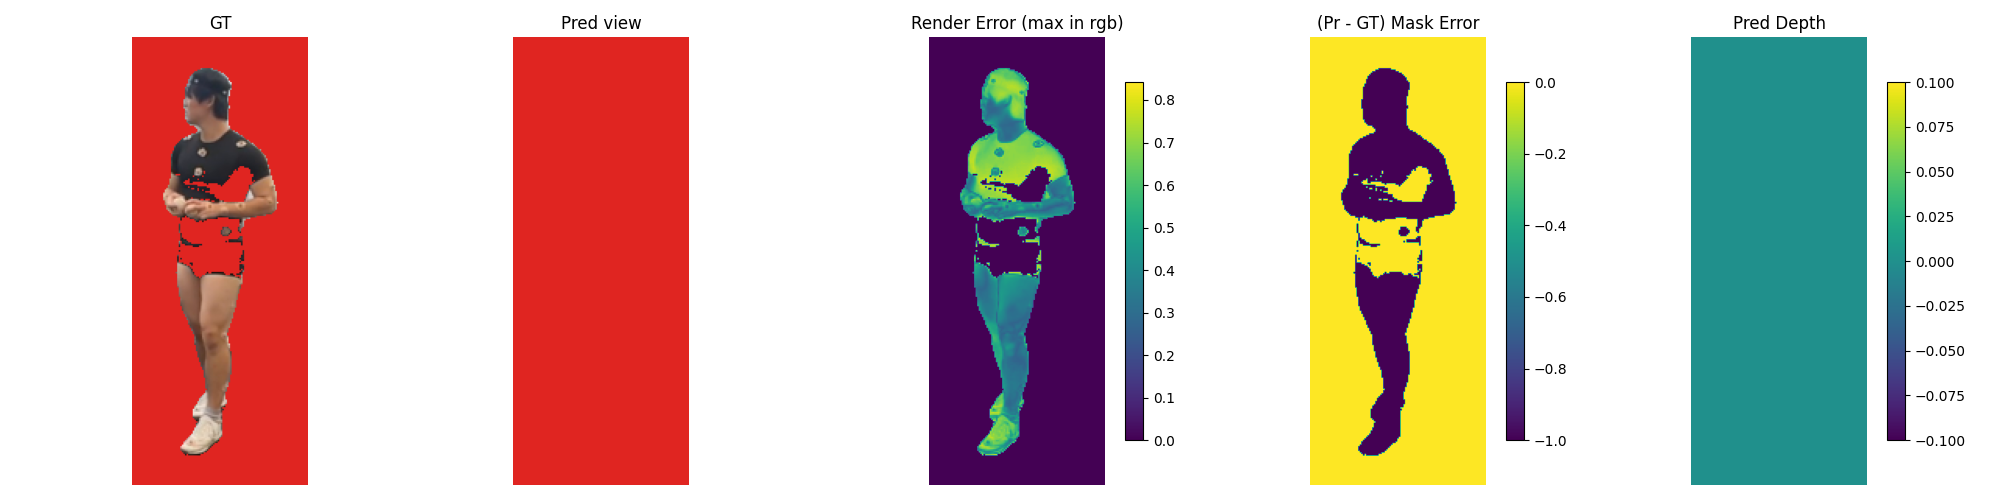
\includegraphics[width=\textwidth]{data/gart_results/step_2999.png}
\caption{GART Step 2999 결과. 좌: GT 이미지, 우: 렌더링. Pred view가 빨간 배경만 나옴 --- SMPL 파라미터가 부정확하여 가우시안이 투수를 재구성하지 못함. Depth 맵에서 실루엣은 보임.}
\end{figure}

\begin{warningbox}
렌더링이 빨간 배경만 나옴. 원인: 배치 피팅 SMPL (reproj 50-135px)이 부정확 + 1뷰만 사용.

해결: U-HMR 999프레임 body\_pose + 7카메라 2D reproj 정제 $\rightarrow$ 정확한 SMPL $\rightarrow$ 7뷰 GART 재학습.
\end{warningbox}


% ====================================================================
\chapter{현재 상태 및 다음 단계}
% ====================================================================

\begin{table}[H]
\centering
\caption{파이프라인 진행 상황}
\renewcommand{\arraystretch}{1.4}
\begin{tabular}{c p{5cm} c p{4cm}}
\toprule
\textbf{Step} & \textbf{작업} & \textbf{상태} & \textbf{비고} \\
\midrule
1 & Conda 환경 분리 (uhmr + gart) & \textbf{완료} & cuDNN, pytorch3d 정상 \\
2 & OpenPose 마스킹 + smoothing & \textbf{완료} & 7대, 1000프레임, v2 \\
3 & U-HMR 전체 프레임 (4뷰) & \textbf{완료} & 999프레임, 18분 \\
4 & 7카메라 2D reproj 정제 & 대기 & U-HMR body\_pose 초기값 \\
5 & GART 7뷰 재학습 & 대기 & Step 4 결과 필요 \\
6 & 생체역학 분석 & 대기 & SMPL2AddBiomechanics \\
\bottomrule
\end{tabular}
\end{table}

\begin{summary}
\textbf{핵심 성과}:
\begin{enumerate}[leftmargin=*]
  \item Conda 환경 분리로 패키지 충돌 해결
  \item U-HMR 999프레임 $\times$ 4뷰 추론 완료 (프레임별 body\_pose)
  \item GART 설치 성공 (smplx 호환성 모두 해결)
  \item GART 첫 학습 완료 (3000 steps, 3분)
  \item OpenPose 마스킹 + 4단계 smoothing (떨림 83-87\% 감소)
\end{enumerate}

\textbf{남은 과제}:
\begin{enumerate}[leftmargin=*]
  \item U-HMR body\_pose + 7카메라 2D reproj $\rightarrow$ 정확한 SMPL 파라미터
  \item 7뷰 ZJU-MoCap 데이터 준비 + GART 재학습
  \item 렌더링 결과가 투수와 일치하는지 검증
\end{enumerate}
\end{summary}


\end{document}
